% ****** Start of file apssamp.tex ******
%
%   This file is part of the APS files in the REVTeX 4 distribution.
%   Version 4.0 of REVTeX, August 2001
%
%   Copyright (c) 2001 The American Physical Society.
%
%   See the REVTeX 4 README file for restrictions and more information.
%
% TeX'ing this file requires that you have AMS-LaTeX 2.0 installed
% as well as the rest of the prerequisites for REVTeX 4.0
%
% See the REVTeX 4 README file
% It also requires running BibTeX. The commands are as follows:
%
%  1)  latex apssamp.tex
%  2)  bibtex apssamp
%  3)  latex apssamp.tex
%  4)  latex apssamp.tex
%
\documentclass[prb,aps,twocolumn,preprintnumbers,amsmath,amssymb]{revtex4}
%\documentclass[preprint,showpacs,preprintnumbers,amsmath,amssymb]{revtex4}

% Some other (several out of many) possibilities
%\documentclass[preprint,aps]{revtex4}
%\documentclass[preprint,aps,draft]{revtex4}
%\documentclass[prb,twocolumn,showpacs,preprintnumbers,amsmath,amssymb]{revtex4}% Physical Review B

\usepackage{graphicx}% Include figure files
\usepackage{dcolumn}% Align table columns on decimal point
\usepackage{bm}% bold math
\usepackage[utf8]{inputenc}
\usepackage{url}
\newcolumntype{P}[1]{>{\centering\arraybackslash}p{#1}}
\newcolumntype{M}[1]{>{\centering\arraybackslash}m{#1}}
%\nofiles

\begin{document}

\title{Difracción de electrones}% Force line breaks with \\

\author{Alejandro Hernández A.}%
 \email{a.hernandez105@uniandes.edu.co}
\author{Daniel Sánchez M.}%
 \email{d.sanchez462@uniandes.edu.co}
\affiliation{%
Departamento de Física\\ Universidad de los Andes, Bogotá, Colombia.\\
}%

\date{10 de septiembre de 2015}% It is always \today, today,
             %  but any date may be explicitly specified

\begin{abstract}
Este informe presenta los datos obtenidos al medir el diámetro de los circulos producidos en el patrón de interferencia de los electrones de un cátodo caliente al ser difractados por una red policristalina de grafito. Con la medición de los diámetros de los círculos del patrón de interferencia se determinaron las distancias interplanares en los cristales de grafito $d_{1} = (1.68 \pm 0.12) \cdot 10^{-10}\ m$ y $d_{2} = (1.07 \pm 0.69) \cdot 10^{-10}\ m$ con errores pocentuales de $E_{1} = 21.13\%$ y $E_{1}= 13.00\%$, y también se halló un valor experimental para la constante de Plank $h = (7.99 \pm 0.56) \cdot 10^{-34} m^2kg/s$ con error porcentual $E = 20.51\%$. Los motivos para errores tan altos serán discutidos en la sección de \textbf{RESULTADOS Y ANÁLISIS}.\\

\noindent \textbf{Conceptos clave:} Difracción, condición de Bragg, relción de De Broglie, conservación de energía.
\end{abstract}
                             
\maketitle

\section{Introducción.}

La dualidad onda-partícula alude al hecho de que todas las partículas elementales exhiben propiedades tanto de partículas como de ondas. Iniciadas por Louis de Broglie, las orígenes de las ideas de dualidad se remontan al debate entre Cristiaan Huygens e Isaac Newton, quienes proponían que la luz consistía de ondas o de partículas respectivamente. Y a través del trabajo de físicos como Max Plank, Albert Einstein, el propio Louis de Broglie, Arthur Compton, Niels Bohr y muchos otros, dicha dualidad es uno de los hechos fundamentales de la ciencia actual y ha sido verificada no solo para partícilulas puntuales sino también para átomos e incluso moléculas.\\

Uno de los ejemplos clásicos de la dualidad onda-partícula se presenta en la difracción de un haz coherente de electrones contra un blanco de características apropiadas, puesto que de esta forma se puede evidenciar un partrón de difracción imposible de explicar sin los características ondulatorias de dichas partículas.\\

Precisamente, en esta práctica de laboratorio se pretende estudiar la difracción de un haz de electrones por una red policristalina de grafito. Luego de pasar por un diagrama de pines y un sistema de enfoque óptico-electrónico, los electrones emitidos por un cátodo caliente inciden en forma de un haz monocrómático muy limitado en una lámina policrisalina de grafito. Para que los electrones sean emitidos se requiere de un potencial $V$ que acelere los electrones y por sonservación de la energía tenemos que:
 
\begin{equation}
\label{conservation}
e \cdot V = \frac{p^{2}}{2m}
\end{equation}

Donde $p$ es el momento lineal del electrón. Luego,\\

\begin{equation}
\label{momento}
p = \sqrt{2meV}
\end{equation}

y al utilizar la relación de de Broglie

\begin{equation}
\label{broglie}
\lambda = \frac{h}{p} = \frac{h}{\sqrt{2meV}}
\end{equation}

\begin{figure}[h!]
	\centering
	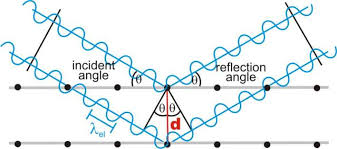
\includegraphics[width=0.4\textwidth]{bragg}
	\caption{ Condición de Bragg. }
	\label{fig: bragg}
\end{figure}

Por otra parte, a partir de la relación de Bragg tenemos que para una disposición regular de átomos en un cristal tenemos que habrá interferencia constructiva en los planos reticulares individuales como los de la figura \ref{fig: bragg}\footnote{Imagen obtenida de http://www.xtal.iqfr.csic.es/Cristalografia\\/parte\_05\_5-en.html\\} si se satisface:

\begin{equation}
\label{bragg}
2 d \sin \theta = n \lambda \ \ \ \ n \in \mathbb{N}
\end{equation}

Donde $d$ es la distacia reticular interplanar y $\theta$ es el ángulo de difracción del rayo incidente con longitud de onda $\lambda$. La ecuación \eqref{bragg} indica que solo se produce interferencia constructiva si la diferencia de camino entre los rayos reflejados es un múltiplo entero entre las longitudes de onda del rayo incidente.\\

Dado a que el material (grafito), a usar en este experimento es policristalino, siempre \footnote{Información obtenida de la guía de laboratorio.\\} hay algunos cristales en los que se satisface la condición de Bragg. Además, las reflexiones producidas por estos dichos cristales quedan en conos cuyo eje común está dado por la dirección de incidencia. De ahí que aparezcan círculos concéntricos en una pantalla ubicada perpendicular a este eje. Y a partir de la figura \ref{fig: montaje} \footnote{Imagen obtenida de la guía de laboratorio porporcionada por el profesor.\\} se puede deducir:

\begin{equation}
\label{eq. 1}
\tan 2\theta = \frac{D}{2L}
\end{equation}

\begin{figure}[h!]
	\centering
	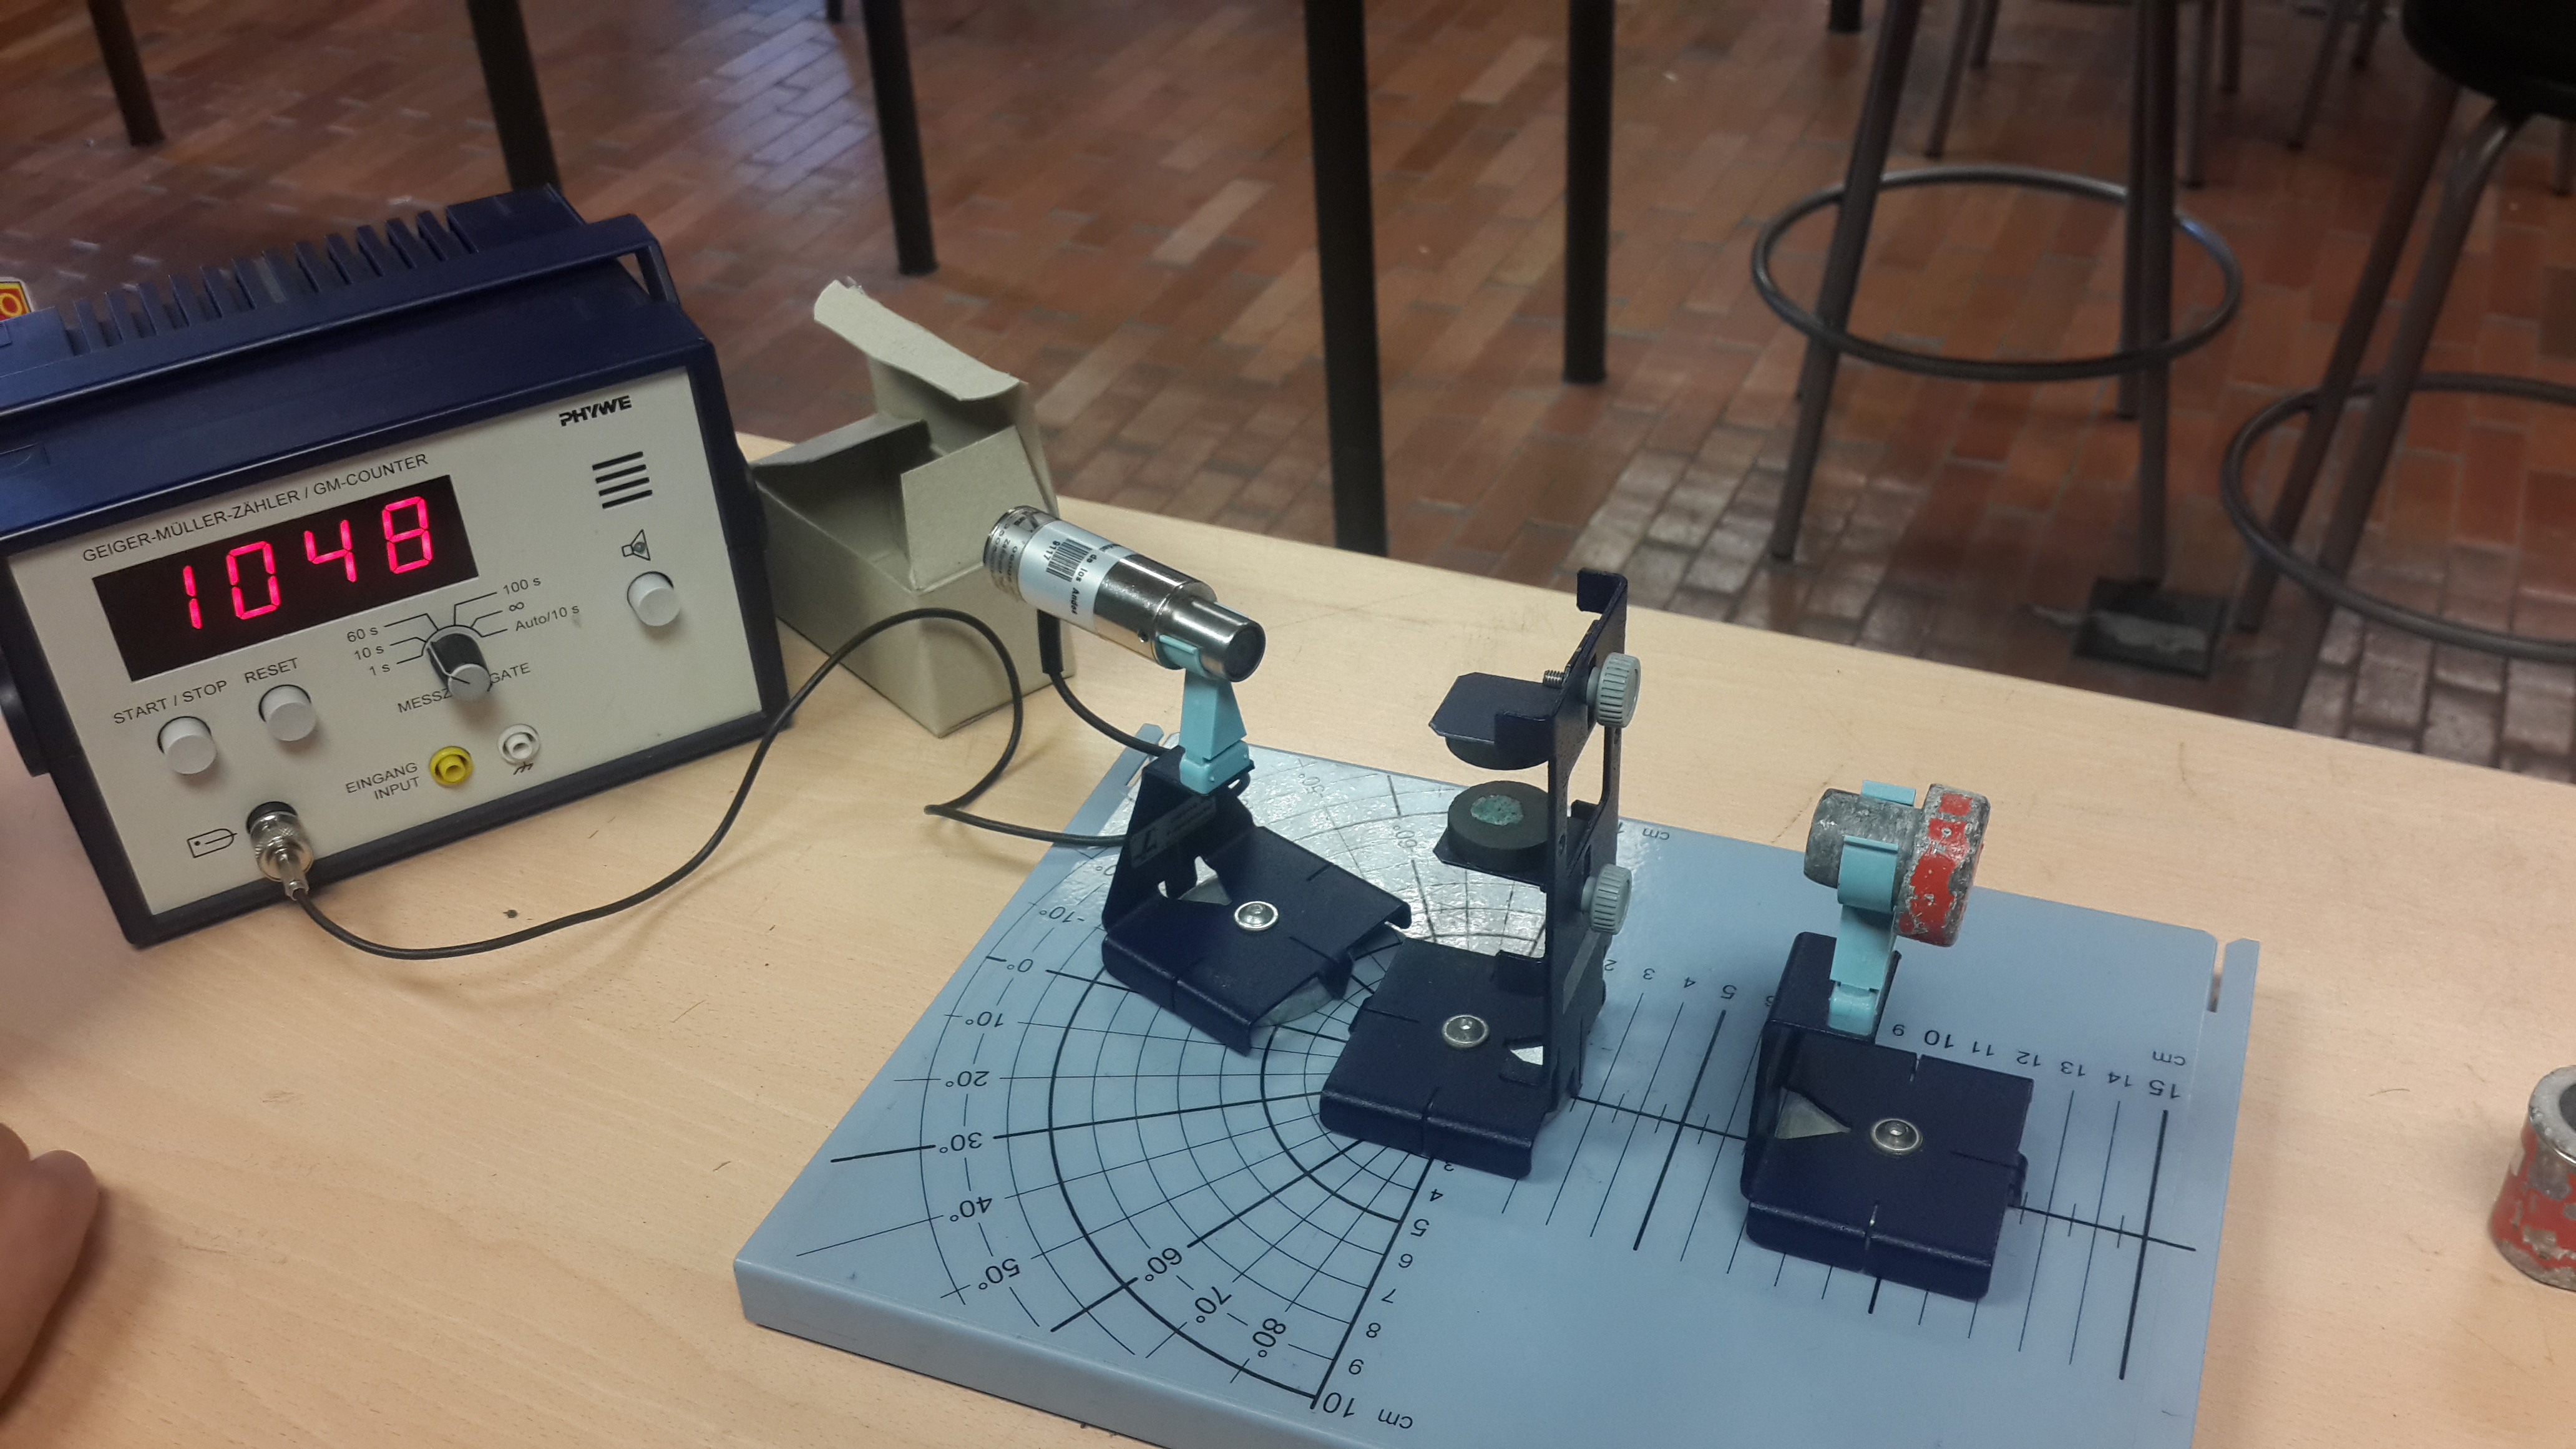
\includegraphics[width=0.4\textwidth]{montaje}
	\caption{ Montaje experimental. }
	\label{fig: montaje}
\end{figure}

Partiendo de la ecuación \eqref{eq. 1}, para ángulos pequeños tenemos que $2 \sin \theta =\frac{D}{2L}$ y al sustituir en \eqref{bragg} con $n = 1$ tenemos:

\begin{equation}
\label{long. onda}
\lambda = d\frac{D}{2L}
\end{equation}

Con $D$ el diámetro del anillo de difracción observado y $L$ la distancia entre el grafito y la pantalla. Finalmente, al combinar las ecuaciones \eqref{bragg} y \eqref{long. onda} obtenemos:

\begin{equation}
\label{diametro}
D = \frac{2Lh}{d\sqrt{2me}} \frac{1}{\sqrt{V}}
\end{equation}

Todas las ecuaciones anteriores serán usadas posteriormente para el análisis de datos teniendo en cuenta que las longitudes de onda teóricas estarán dadas por \eqref{broglie} y las longitudes de onda experimentales por \eqref{long. onda}. 

\section{Montaje experimental}

Los elementos usados durante la práctica fueron los siguientes:

\begin{itemize}
	\item Un tubo de difracción de electrones.
	\item Un portatubo.
	\item Una fuente de alimentación de alta tensión de $10\ kV$.
	\item Un calibre Vernier de alta precisión.
	\item Diversos cables de conexión.
\end{itemize}

Tal como se muestra en la figura \ref{fig: montaje2}\footnote{Imagen obtenida de la guía de laboratorio proporcionada por el profesor.\\}, la forma de realizar las conexiones se menciona a continuación \footnotemark[4].

\begin{itemize}
	\item Primero conectamos los enchufes hembra para calentar el cátodo F1 y F2 del portatubo a la salida en la parte trasera de la	fuente de alimentación de alta tensión de 10 kV. 
	
	\item Luego conectamos los enchufes hembra C (tapa del cátodo) y X
	(electrodo de enfoque) del portatubo al polo negativo. 
	
	\item Posteriormente conectamos el enchufe hembra A (ánodo) al polo positivo de	la salida de 5 kV/2 mA de la fuente de alimentación de
	alta tensión de 10 kV.
	
	\item Finalmente, conectamos a tierra el polo positivo de la fuente
	de alimentación de alta tensión de 10 kV. 
	
\end{itemize}

\begin{figure}[h!]
	\centering
	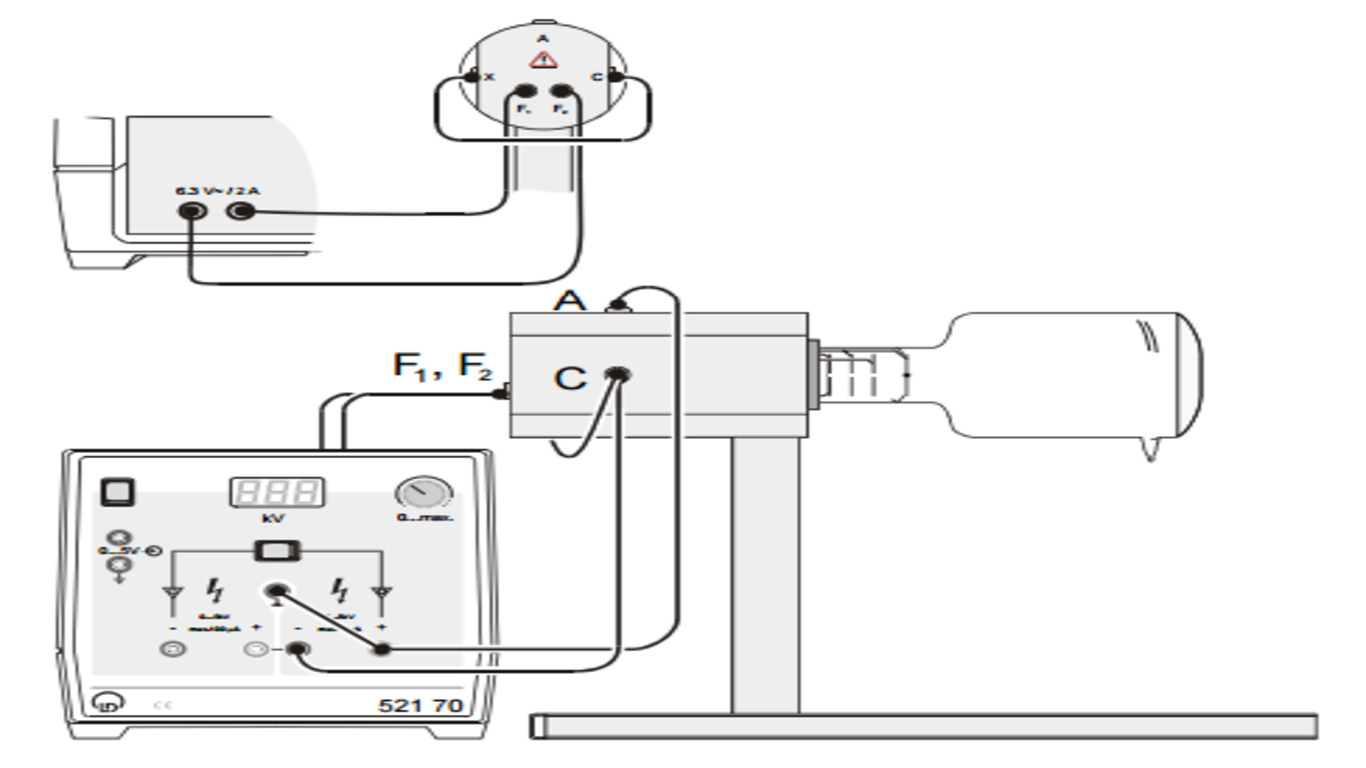
\includegraphics[width=0.4\textwidth]{montaje2}
	\caption{ Forma de realizar las conexiones. }
	\label{fig: montaje2}
\end{figure}

La idea del experimento era observar dos círculos de difración causados por una especie de doble rendija en una lámina de grafito. Particularmente, los pasos a seguir para hacer las meddiciones fueron los siguientes:

\begin{itemize}
	\item Con el fin de familiarizarnos con el funcionamiento de lo instrumentos proporcionados, colocamos un voltaje no mayor a $5\ kV$ y observamos los dos círculos del patrón de difracción. 
	
	\item Habiendo hecho lo anterior, procedimos a variar el voltaje de aceleración entre $3\ kV$ y $5\ kV$ y medimos los diámetros de ambos círculos o anillos de difracción.
	
	\item Finalmente, medimos la distancia entre la lámina de grafito y la pantalla en la cual se observaban los círculos.
\end{itemize}

\section{Resultados y análisis}

Los resultados de las mediciones realizadas se muestran a continuación

\begin{table}[h!]
	\caption{\label{Tabla 1}Diámetros de los anillos de difracción.}
	\begin{ruledtabular}
		\begin{tabular}{|ccc|}
			Voltaje ($V$ ) & $(D_{1} \pm 0.005)(cm)$ & ($D_{2}\ \pm 0.005)(cm)$\\
			\hline
			3.0 & 3.15 & 5.30\\
			3.2 & 2.90 & 4.85\\
			3.4 & 2.76 & 4.75\\
			3.6 & 2.74 & 4.55\\
			3.8 & 2.55 & 4.40\\
			4.0 & 2.50 & 4.25\\
			4.2 & 2.45 & 4.20\\
			4.4 & 2.36 & 4.12\\
			4.6 & 2.34 & 4.11\\
			4.8 & 2.31 & 3.92\\
			5.0 & 2.30 & 3.88\\
		\end{tabular}
	\end{ruledtabular}
\end{table}
\
\\\\\\\\\\

Cabe aclarar que la incertidumbre de los datos de los diámetros está dada por la incertidumbre del calibrador. La distancia medida	de la lámina de grafito y la pantalla fue de $L = 13.68\ cm$. Teniendo en cuenta lo anterior y las ecuaciones \eqref{broglie} y \eqref{long. onda}, las longitudes de onda obtenidas para cada uno de los anillos se muestran en las tablas \ref{Tabla 2} y \ref{Tabla 3}.

\begin{table}[h!]
	\caption{\label{Tabla 2}Longitudes de onda experimentales y teóricas para el círculo interno.}
	\begin{ruledtabular}
		\begin{tabular}{|cccc|}
			$V$ & $(D_{1} \pm 0.005)(cm)$ & $\lambda_{teo}\ (10^{-11}\ m)$ & $\lambda_{exp}\ (10^{-11}\ m)$\\
			\hline
			3.0 & 3.15 & 2.23 & 2.45\\
			3.2 & 2.90 & 2.16 & 2.26\\
			3.4 & 2.76 & 2.10 & 2.15\\
			3.6 & 2.74 & 2.04 & 2.13\\
			3.8 & 2.55 & 1.98 & 1.98\\
			4.0 & 2.50 & 1.93 & 1.94\\
			4.2 & 2.45 & 1.89 & 1.91\\
			4.4 & 2.36 & 1.84 & 1.84\\
			4.6 & 2.34 & 1.81 & 1.82\\
			4.8 & 2.31 & 1.77 & 1.80\\
			5.0 & 2.30 & 1.73 & 1.79\\
		\end{tabular}
	\end{ruledtabular}
\end{table}

\begin{table}[h!]
	\caption{\label{Tabla 3}Longitudes de onda experimentales y teóricas para el círculo externo.}
	\begin{ruledtabular}
		\begin{tabular}{|cccc|}
			$V$ & $(D_{2} \pm 0.005)(cm)$ & $\lambda_{teo}\ (10^{-11}\ m)$ & $\lambda_{exp}\ (10^{-11}\ m)$\\
			\hline
			3.0 & 5.30 & 2.23 & 2.38\\
			3.2 & 4.85 & 2.16 & 2.18\\
			3.4 & 4.75 & 2.10 & 2.13\\
			3.6 & 4.55 & 2.04 & 2.04\\
			3.8 & 4.40 & 1.98 & 1.99\\
			4.0 & 4.25 & 1.93 & 1.91\\
			4.2 & 4.20 & 1.89 & 1.88\\
			4.4 & 4.12 & 1.84 & 1.85\\
			4.6 & 4.11 & 1.81 & 1.84\\
			4.8 & 3.92 & 1.77 & 1.76\\
			5.0 & 3.88 & 1.73 & 1.74\\
		\end{tabular}
	\end{ruledtabular}
\end{table}

Es importante resaltar que al hacer propagación de error \footnotemark[3] sobre los datos de cada tabla encontramos que el error en las medidas fue de $\Delta \lambda_{1} = 0.13  \cdot 10^{-11} m$ y $\Delta \lambda_{2} = 0.07 \cdot 10^{-11} m$.\\

Ahora bien, en esta instancia es posbile afirmar que se pudo verificar el cumplimiento de la relación de de Broglie para los electrones, dada la gran cercarnía de los datos teóricos con los experimentales, además, al calcular la máxima diferencia entre los datos teóricos y los datos experimentales tanto para el círculo interno como para el círculo externo se obtuvieron resultados del orden de $10^{-12} m$, un orden de magnitud por debajo de los datos obtenidos, permintiendo confirmar nuevamente el cumplimiento de la relación de de Broglie para los electrones.\\

Ahora bien, para determinar las distanicias interplanares se usó la ecuación \eqref{diametro} de la siguiente manera:

\begin{equation}
\label{diametro2}
\frac{2Lh}{\sqrt{2me}} \frac{1}{\sqrt{V}} = dD
\end{equation}

Y haciendo un fit de los datos para los valores tanto del diámetro interno como del diámetro externo se halló que las ditancias interplanares experimentales fueron:

\begin{equation}
\label{interplanar}
\begin{split}
d_{1} &= (1.68 \pm 0.12 )\cdot 10^{-10}\ m\\
d_{2} &= (1.07 \pm 0.69 )\cdot 10^{-10}\ m
\end{split}
\end{equation}

Los cuales, en comparación con los datos teóricos $d_{1} = 2.13 \cdot 10^{-10}\ m$ y $d_{2} = 1.23 \cdot 10^{-10}\ m$ tienen errores porcentuales de $21.13\%$ y $13.00\%$ respectivamente. Estos errores relativamente altos se deben pricipalmente a que la pantalla sobrela cual se observaban los cículos era curva, lo cual hacía difícil e inprecisa la toma de datos. Además, los anillos no eran perfectamente nítidos sobre la pantalla, es decir, no se observaban como una línea definida sino que tenían cierto grosor, y a pesar de que se intentó siempre tomar datos justo en la "mitad" de dicho grosor, esto no siempre fue posible.\\

Finalmente, teniendo todos los datos anteriores, es posible estimar el valor de la constante de Plank, usando nuevmente la ecuación \eqref{diametro}, despejando esta vez para $h$ y usando los valores experimentales de las distancias interplanares. Los valores obtenidos fueron los siguientes:

\begin{equation}
\label{plank}
\begin{split}
h_{d_{1}} &= (8.37 \pm 0.62) \cdot 10^{-34}\ m^2kg/s\\
h_{d_{2}} &= (7.61 \pm 0.51) \cdot 10^{-34}\ m^2kg/s
\end{split}
\end{equation}

Y en promedio tenemos que $h_{exp} = (7.99 \pm 0.56) \cdot 10^{-34}\ m^2kg/s$ que si bien tiene el orden de magnitud correcto con respecto al valor teórico $h = 6.63 \cdot 10^{-34}\ m^2kg/s$ tiene un error porcentual de $20.51\%$. Dicho error también puede ser explicado en términos de los mencionados previamente y por la propagación de los mismos, puesto que para determinar el valor experimental de $h$ se usaron los datos previamente obtenidos de las distancias interplanares. Cabe realtar que si bien obtuvimos un error porcentual superior al $20\%$, dicho error es de esperarse dado a que estábamos tratando de determinar indirectamente una constante extremadamente pequeña mediante un método que no era lo suficientemente exacto dados los errores mencionados previamente.

\section{Conclusiones}

\begin{itemize}

	\item Se lograron verificar el cumplimiento de la relación de de Broglie para los electrones tanto visualmente como numéricamente, ya que seria imposible haber observado el patrón de difracción sin las características ondulatorios de dichas partículas, además de que los datos experimentales de las longitudes de onda coinciden relativamente bien con los datos teóricos.
	
	\item Se lograron hallar las distancias interplanares del grafito $d_{1} = (1.68 \pm 0.12 )\cdot 10^{-10}\ m$ y $d_{2} = (1.07 \pm 0.69 )\cdot 10^{-10}\ m.$ con errores porcentuales altos debidos a las dificultades para tomar los datos de los diámetros de los anillos de difracción.
	
	\item Se logró hallar indirectamente un valor experimental para la constante de Plank $h_{exp} = (7.99 \pm 0.56) \cdot 10^{-34}\ m^2kg/s$, que si bien tiene el orden de magnitud correcto, tiene un error porcentual de $20.52\%$. Cabe mencionar que la mayor fuente de error para esta constante es la propagación de los errores mencionados en el análisis de datos.
		
	\item Lo más importante que pudimos notar en el experimento fue que la dificultad de la curvatura de la pantalla experimentada al realizar las mediciones del diámetro fue la mayor fuente de error del experimento, y una posible forma de reducir este error sería repitiendo el experimento múltiples veces con el fin de tener una medida promedio de los diámetros.
	
\end{itemize}

\begin{thebibliography}{99}
\
\\
\bibitem{french} A. P. French, {\it Vibrations and Waves}{, The MIT Introductory Physics Series, USA, 1960}.\\
\bibitem{Tipler} Tipler, Paul A., \textit{Physics for scientists and engineers}. W.H. Freeman, 4 Edici\' on, 1999.\\
\bibitem{Taylor} Taylor, J.R., \textit{An Introduction to Error Analysis}. University Science Books, Sausalito, California. 2nd edition, 1982.\\
\end{thebibliography}

\end{document}
%
% ****** End of file apssamp.tex ******
